\section{UDP}

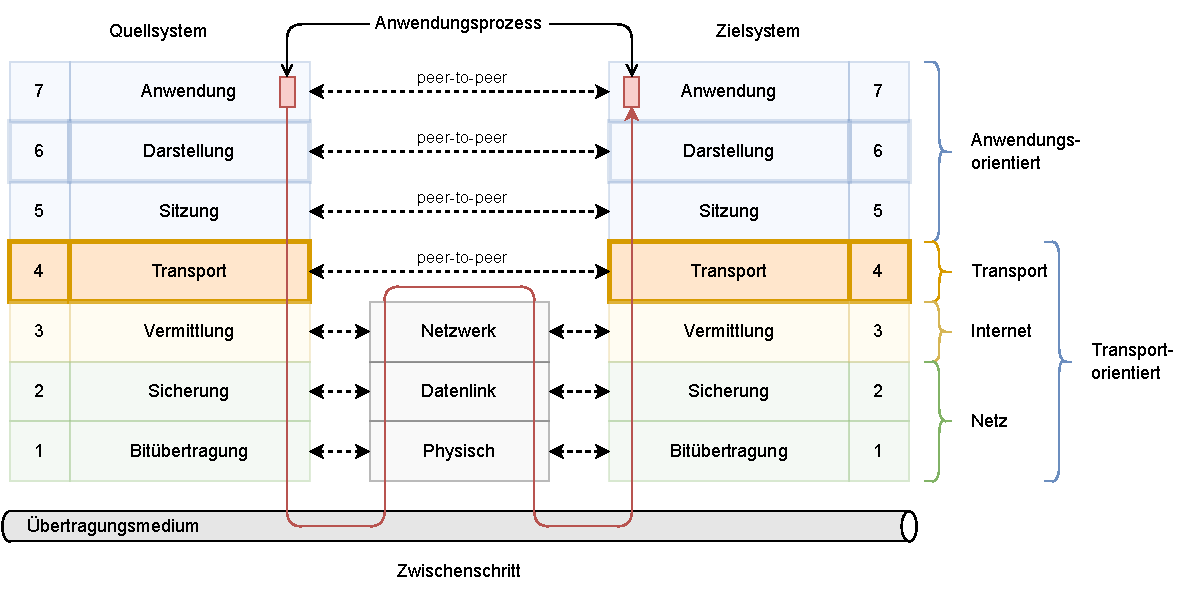
\includegraphics[width=\textwidth]{includes/figures/defi_iso_osi_transport.pdf}

\begin{defi}{UDP}
    Das \emph{User Datagram Protocol (UDP)} ist ein \emph{verbindungsloses, nicht-zuverlässiges und ungesichertes wie auch ungeschütztes} Netzwerkprotokoll, das zur Transportschicht der Internetprotokollfamilie gehört.

    UDP ermöglicht den Versand von Datagrammen in IP-basierten Rechnernetzen.

    UDP verwendet Ports, um versendete Daten dem richtigen Programm auf dem Zielrechner zukommen zu lassen.
    Dazu enthält jedes Datagramm die Portnummer des Dienstes, der die Daten erhalten soll.

    Zusätzlich bietet UDP die Möglichkeit einer Integritätsüberprüfung an, indem eine Prüfsumme mitgesendet wird.
    Dadurch können fehlerhaft übertragene Datagramme erkannt und verworfen werden.

    Daneben bietet die ungesicherte Übertragung den Vorteil von geringen Übertragungsverzögerungsschwankungen: Geht bei einer TCP-Verbindung ein Paket verloren, wird es automatisch neu angefordert.
    Das braucht Zeit, die Übertragungsdauer kann daher schwanken, was für Multimediaanwendungen schlecht ist.
    Bei VoIP (Discord, MS Teams) oder Streaming (Netflix, YouTube) z. B. käme es zu plötzlichen Aussetzern, bzw. die Wiedergabepuffer müssten größer angelegt werden. Bei verbindungslosen Kommunikationsdiensten bringen verlorengegangene Pakete dagegen nicht die gesamte Übertragung ins Stocken, sondern vermindern lediglich die Qualität.
\end{defi}

\begin{defi}{UDP-Header}
    \begin{center}
        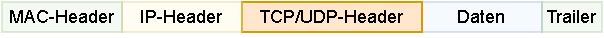
\includegraphics[width=0.75\textwidth]{includes/figures/defi_tcp_header_kapselung.pdf}

        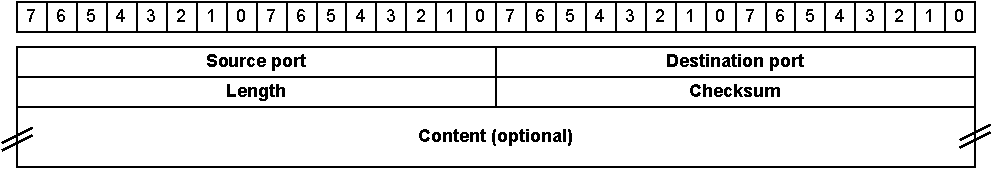
\includegraphics[width=0.75\textwidth]{includes/figures/defi_udp_header.pdf}
    \end{center}
\end{defi}

\begin{bonus}{Abtastung}
    Analoge Signale werden regelmäßig gemessen.

    Dabei wird der Wert zu dem n-ten Zeitpunkten $t_n = n \cdot \Delta t$ gemessen.

    Bei dem \texttt{Hold}-Verfahren wird der letzte gemessene Wert gehalten:

    \begin{center}
        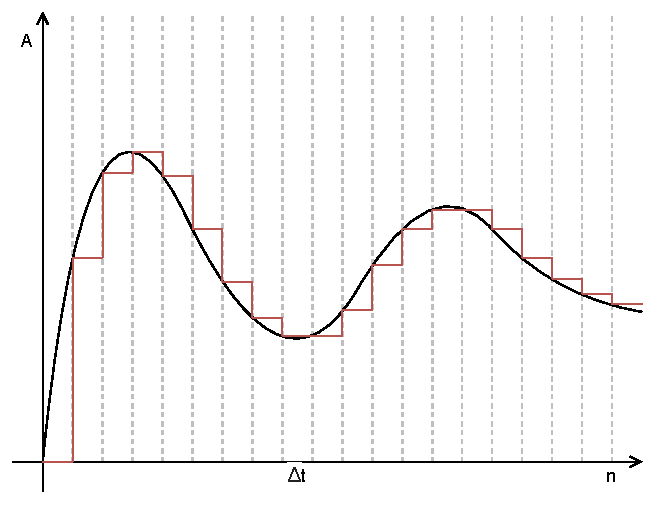
\includegraphics[width=0.5\textwidth]{includes/figures/defi_abtastrate.pdf}
    \end{center}
\end{bonus}

\begin{defi}{Sampling Rate}
    \begin{itemize}
        \item Wird zu selten abgetastet, erhalten wir eine sehr ungenaue Approximation des ursprünglichen analogen Signals

              \begin{center}
                  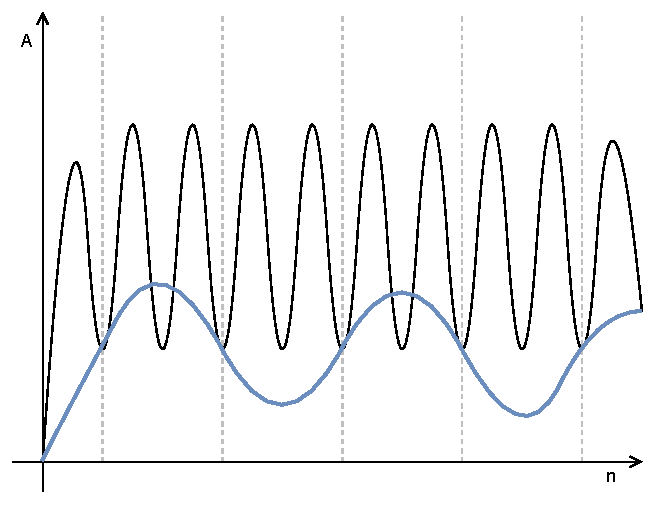
\includegraphics[width=0.5\textwidth]{includes/figures/defi_sampling_rate_error.pdf}
              \end{center}
        \item Wird zu häufig abgetastet, verbrachen wir Ressourcen, die eventuell für unseren Anwendungsfall nicht genutzt werden müssten
    \end{itemize}

    Nach den \emph{Nyquist-Shannon-Abtasttheorem} soll gelten: $\text{Abtastrate} > 2 \cdot \text{max. Frequenz}$
\end{defi}

\begin{bonus}{Quantisierung und Kodierung}
    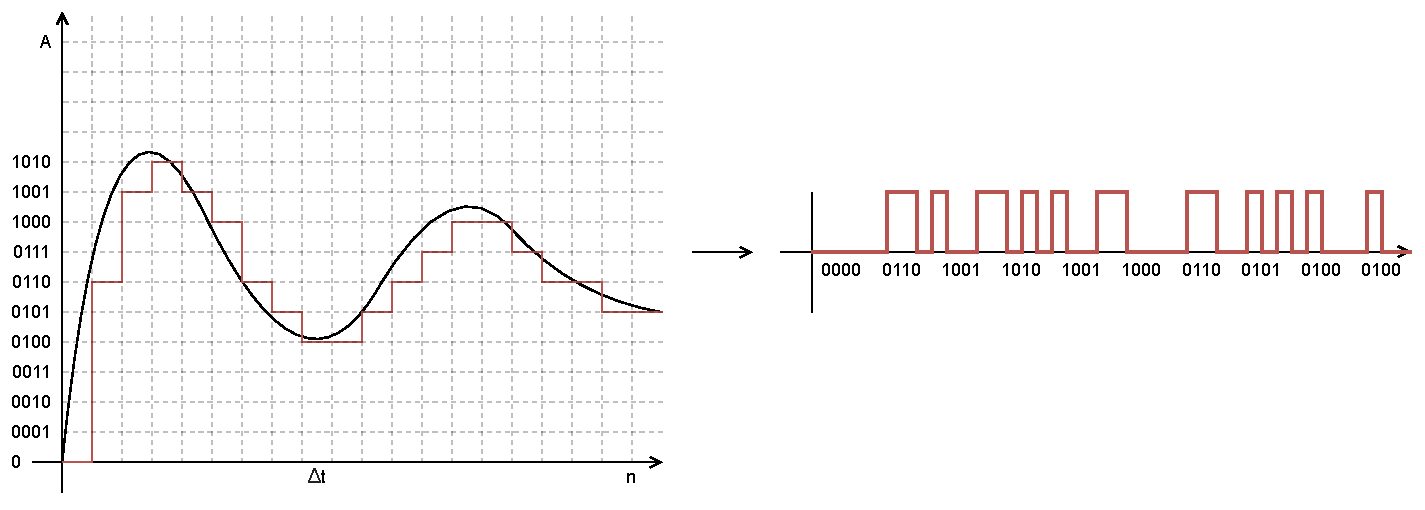
\includegraphics[width=\textwidth]{includes/figures/defi_quantisierung.pdf}

    Das Analoge Signal wird \emph{quantisiert} (umgewandelt) und danach in digitale Werte kodiert.
\end{bonus}

\begin{defi}{RTP}
    Das RTP-Protokoll liefert Transportschnittstellen, die UDP erweitern:
    \begin{itemize}
        \item UDP liefert Port-Nummern
        \item IP die Adressen der Endpunkte
        \item \texttt{RTCP} liefert Statistiken auf UDP-Basis
        \item \texttt{RTSP} ist die \enquote{Fernbedienung}
    \end{itemize}

    \begin{center}
        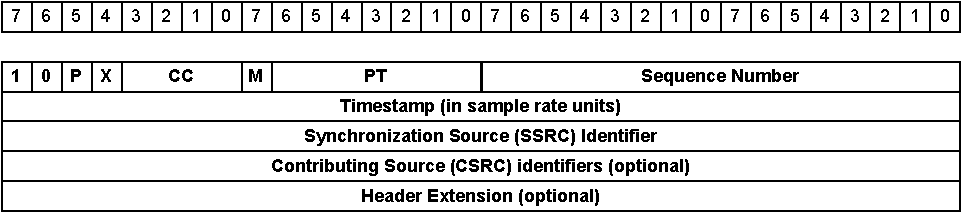
\includegraphics[width=0.75\textwidth]{includes/figures/defi_rtp.pdf}
    \end{center}
\end{defi}
